\subsection{Isosurface Extraction}\label{sec:isocontour}

% \begin{figure}[t]
% \centering
% \subcaptionbox{\emph{by bit plane} (\sbit)}
% {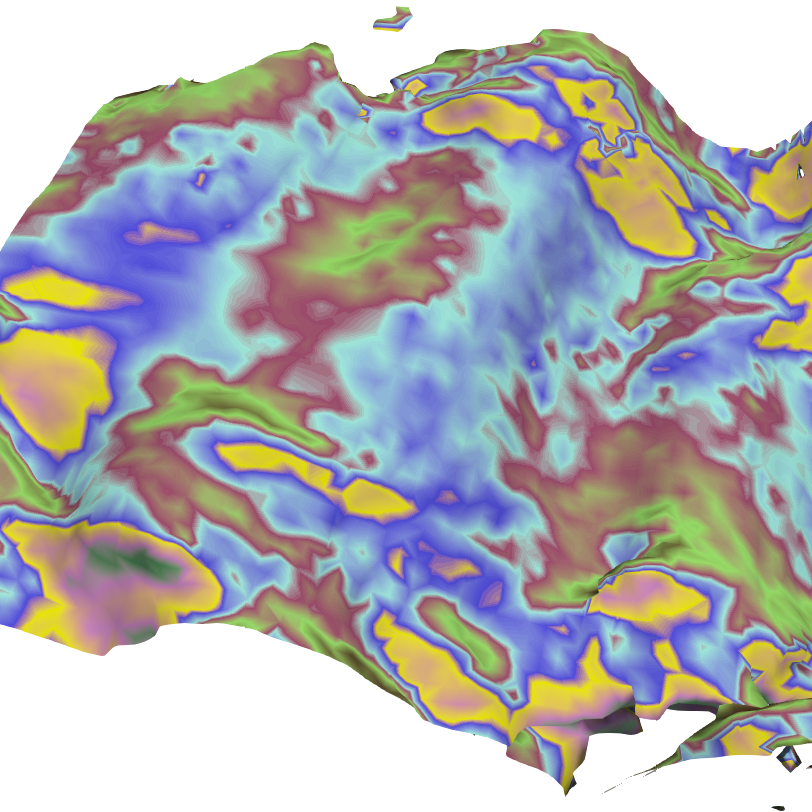
\includegraphics[width=0.32\linewidth]{isocontour/isocontour2-bit-plane}}
% \subcaptionbox{\emph{by wavelet norm} (\swav)}
% {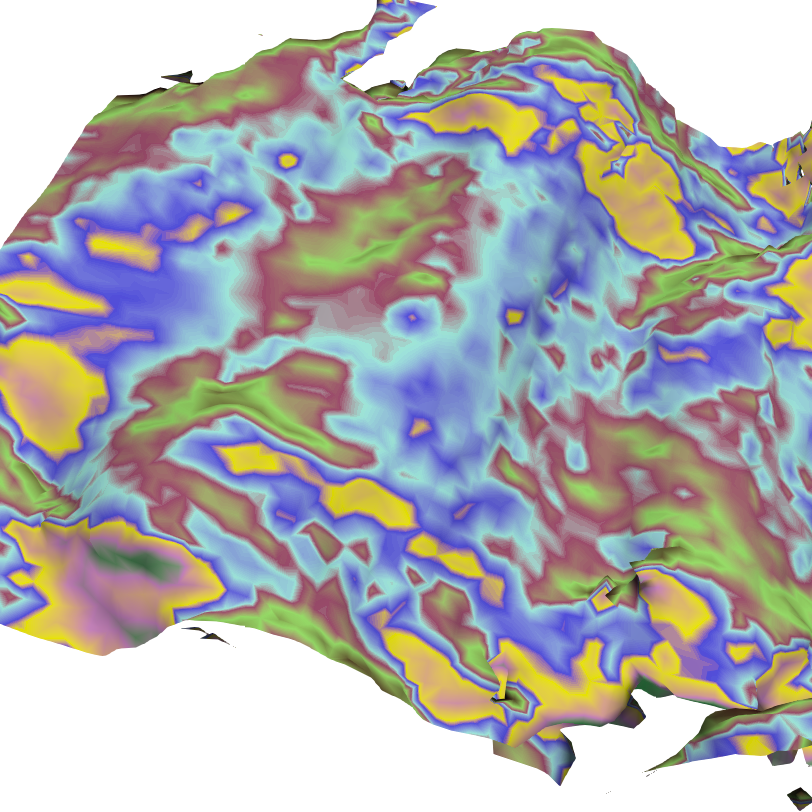
\includegraphics[width=0.32\linewidth]{isocontour/isocontour2-wavelet-norm}}
% \subcaptionbox{\emph{ground truth}}
% {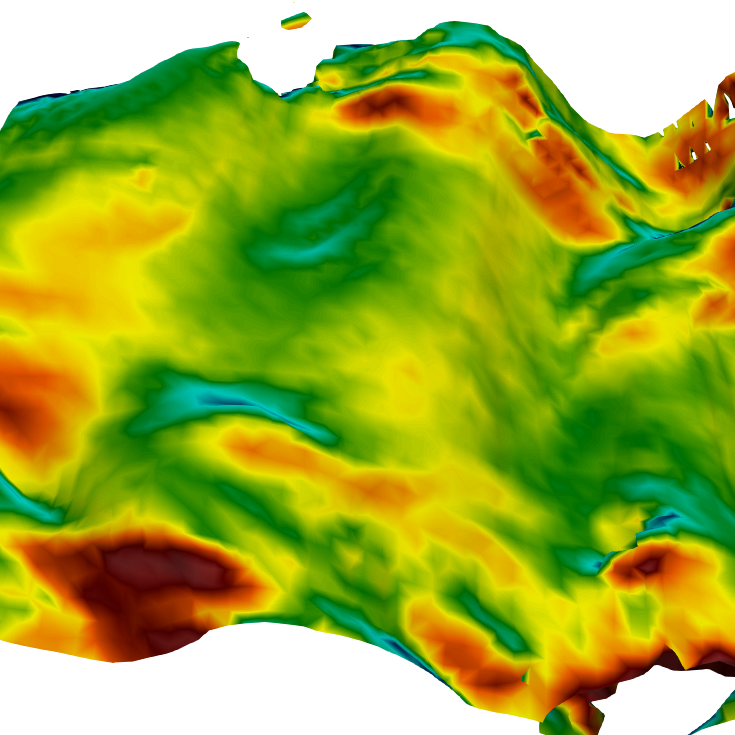
\includegraphics[width=0.32\linewidth]{isocontour/isocontour2-groundtruth}}
% \caption{\emph{plasma}'s isosurface reconstructed at 0.5 bps. The surfaces are colored by the
% $x$-component of the normal vectors. The reconstruction by \sbit is closer to the reference (compare
% e.g., yellow features and green features).}
% \label{fig:isocontour-surfaces-plasma}
% \vspace{-1em}
% \end{figure}

\begin{figure}[!b]
\vspace{-1em}
\centering
 \subcaptionbox{\label{fig:bit-distrib-rmse-tile}\emph{RMSE signature}}{{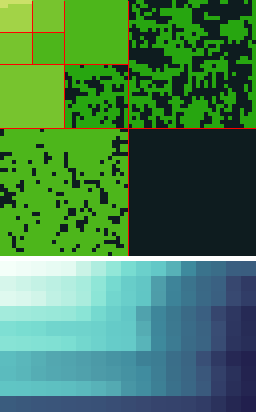
\includegraphics[width=0.32\linewidth]{bit-distrib-rmse-tile}\vspace{-0.5em}}}
 \subcaptionbox{\label{fig:bit-distrib-laplacian-tile}\emph{Laplacian signature}}{{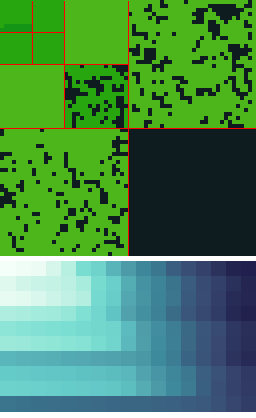
\includegraphics[width=0.32\linewidth]{bit-distrib-laplacian-tile}\vspace{-0.5em}}}
 \subcaptionbox{\label{fig:bit-distrib-histogram-tile}\emph{histogram signature}}{ {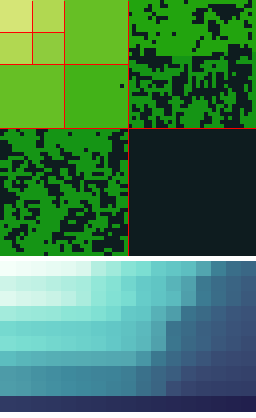
\includegraphics[width=0.32\linewidth]{bit-distrib-histogram-tile}\vspace{-0.5em}}}
 \vspace{-0.5em}
\caption{(Top) Bit distribution across subbands at 1.9 bps for signature-based streams, and (bottom)
corresponding stream signatures. The data is a 2D slice from \emph{diffusivity}. Subbands are
separated by red lines. The color of each pixel indicates the bit plane at which the corresponding
coefficient currently is. Brighter greens correspond to more precision. Both the top and the bottom
rows show that \shsg allocates more bits to the lower subbands, while \slsg prefers to stream bits
from higher subbands. \srsg is somewhere in the middle.}
\label{fig:bit-distrib}
\vspace{-1.5em}
\end{figure}

Studying isosurfaces of a given function is an essential task in many visualization and analysis
pipelines, as they can highlight features of interest. For measuring error between isosurfaces, we
have found that the commonly used Hausdorff distance does not work well in our case, because two
very different reconstructed surfaces may share the same Hausdorff distance to the reference. More
sophisticated metrics exist, focusing on different characteristics such as
geometric~\cite{verifiable-isosurface} and topological~\cite{topology-verification-isosurface}
properties, but they assume the surface has certain properties. Since isosurfaces partition the
domain into ``inside'' and ``outside'' regions, we opt for a simpler error metric that assumes
nothing about the shape of the isosurfaces, but simply counts misclassified voxels. This metric
differs from comparing histograms with two bins in that we care about the spatial position and not
just voxel counts.

However, if the error caused by discarding a packet is of subvoxel resolution, such a metric fails
to capture the importance of that packet, causing \siop to be ineffective. Therefore, we add the
relative difference in surface areas ($|A_1-A_2|/|A_1|$) to the error term. This additional term is
often between $[0, 1]$ and is meant to capture the subvoxel error when the number of misclassified
voxels is zero.

With the error metric defined, we can compute a data-dependent stream optimized for this metric
(\siop) and a stream based on its signature (\sisg) using~\Cref{alg:greedy}
and~\Cref{alg:signature}. \Cref{fig:isocontour-plots} compares the performances of these two
streams, along with \sbit, \slvl, \swav, and \smag. As can be observed, \slvl performs poorly,
indicating that isosurface extraction favors resolution over precision. \emph{plasma} is the only
data set where \sbit outperforms \swav.

\swav typically outperforms \sbit, but \sisg does not provide a clear advantage over \swav as often
seen in other tasks. The reduced effectiveness of \sisg may be explained by the fact that to compute
an isosurface error, voxels are classified into only two broad categories, allowing for a higher
tolerance for differences in streams.~\Cref{fig:isocontour-surfaces-pressure} renders the
isosurfaces reconstructed at 0.6 bps for all streams. In terms of the quality of the reconstructed
surfaces, $\sisg \approx \swav > \sbit > \smag > \slvl$, which agrees with the plots
in~\Cref{fig:isocontour-plots}. For isosurface extraction, \swav seems to be the only stream ---
among the data-independent ones --- that consistently works well in all cases.
